\documentclass[11pt]{article}
\usepackage[a4paper,margin=25mm]{geometry}
\usepackage[T1]{fontenc}
\usepackage{lmodern}
\usepackage{booktabs}
\usepackage{amsmath}
\usepackage{graphicx}
\usepackage{hyperref}
\usepackage{xcolor}
\usepackage{listings}
\lstset{basicstyle=\ttfamily\small, columns=fullflexible, keepspaces=true,
  breaklines=true, frame=single, framerule=0.3pt, rulecolor=\color{gray}}
\newcommand{\code}[1]{\texttt{#1}}
\newcommand{\us}{\textmu s}

\title{\code{template.py}: the shape of the single-photoelectron pulse}
\author{BGOTSCAN}
\date{2026-10-14}

\begin{document}
\maketitle

\section{Purpose}

The single-photoelectron pulses of the SiPMs are 15 counts high and two or
three samples wide (about 20~ns) on 4 counts of white noise per sample. A
threshold on one sample cannot separate them from noise
(\code{spe\_doc.tex}): a matched filter, which uses the shape of the pulse,
is needed, and the shape must be measured first. This script does only
that: it finds the pulse shape, the \emph{template}, from the pulses of
the records, checks it channel by channel, and writes it for
\code{spe.py} to use. It processes one event at a time in seven steps, with
the text and one figure per step, as \code{selection.py} and
\code{spe.py}; the shape needs thousands of pulses, so its normal use is
the \code{--summary} mode over a few hundred events. It is a Python script
in \code{src/py/}, reading the raw HDF5 files with h5py; the shared definitions come from the
package \code{bgo} (\code{bgo\_doc.tex}).

\section{Usage}

\begin{lstlisting}
python3 src/py/template.py RUN [options]
\end{lstlisting}

Interactive: after each step the script waits on the terminal; Enter goes
to the next step, \code{n} abandons the event and starts the next one,
\code{q} quits.

\begin{center}
\begin{tabular}{l l p{74mm}}
\toprule
option & default & meaning \\
\midrule
\code{--data DIR} & the data directory & as in \code{wfview.py} \\
\code{--events SPEC} & \code{0} & events to process: \code{a-b} or \code{a,b,c}, 0-based \\
\code{--channel C} & 0 & the channel shown in steps 1 and 2 \\
\code{--region R} & \code{tail} & search region: \code{tail}, the last \code{--tail} \us{} of the record, or \code{all} \\
\code{--tail T} & 10 & length of the tail region in \us \\
\code{--threshold A} & 12 & candidate threshold on the raw waveform, in ADC counts (3 sigma: high on purpose) \\
\code{--half H} & 8 & half length of the template in samples: $2H + 1$ samples, 136~ns for $H = 8$ \\
\code{--from-step N} & 1 & start the display at this step (1 to 7) \\
\code{--save NAME} & off & no prompts; figures saved as \code{src/py/plots/NAME\_evE\_sN.png} \\
\code{--summary} & off & steps 1 and 2 silent per event; steps 3 to 6 once after the last event (figures saved as \code{NAME\_sN.png} with \code{--save}) \\
\code{--write FILE} & off & write the refined template of step~5 to \code{FILE} as CSV \\
\code{--dead LIST} & the twelve of \code{chanstat\_doc.tex} & channels without signal, used by step~7 as the noise sample \\
\code{--lags K} & 32 & lags of the noise autocorrelation, in samples \\
\code{--pad P} & 8 & zeros added on each side of the template for the whitened filter window ($2H + 1 + 2P$ samples) \\
\code{--write-filter FILE} & off & write the whitened filter weights of step~7 to \code{FILE} as CSV \\
\bottomrule
\end{tabular}
\end{center}

\section{Notation}

$x_i$ is a channel waveform minus its baseline, the median over the
record; $\Delta t = 8$~ns; $R$ is the search region (\code{spe\_doc.tex},
step~1). No common-mode subtraction. A template is a vector $T_j$, $j =
-H \dots H$, normalised to $T_0 = 1$ at the peak.

\section{The steps}

\subsection{Step 1: candidates on the channel}

Candidates are the local maxima of the raw $x$ inside $R$ with $x >
A_{\rm thr}$ (\code{--threshold}, 12 counts), taken in decreasing order
and at least $2H$ samples apart. The threshold is high so that most
candidates are real pulses; the price, pulses lost on the low side, does
not matter here, since only the shape is wanted. Text: number, times and
amplitudes. Figure: $x$ over $R$ with the threshold and the candidates
marked.

\subsection{Step 2: aligned pulses of the channel}

For each candidate at sample $i_A$ (its maximum), the raw samples $x_{i_A
- H} \dots x_{i_A + H}$ minus a local baseline, the median of the window
samples more than two samples before the peak, which removes the slow
wander of the channel at the time of the pulse without being pulled by
the tail of the pulse itself. Text: the number of
pulses. Figure: the pulses
overlaid against the sample offset $j$, and their mean.

\subsection{Step 3: all channels, accumulated}

Steps 1 and 2 on the 64 channels, added to the pulses accumulated over
the events processed so far. Text: pulses per channel as an $8\times8$
table and the total. Figure: a two-dimensional histogram of amplitude
versus offset $j$ over all accumulated pulses, with their mean drawn on
top: the shape with its spread.

\subsection{Step 4: first template}

$T^{(1)}_j$ is the mean of the accumulated pulses at offset $j$, divided
by its value at $j = 0$. Text: the $2H + 1$ values, the full width at
half maximum in samples (linear interpolation between samples), the
undershoot ($\min_{j > 0} T_j$), the sum of squares $\sum_j T_j^2$, and
the standard error of the mean at the peak. Figure: $T^{(1)}$ with the
standard error of each sample.

The sum of squares is what the matched filter gains. For a pulse of
shape $T$ on white noise $\sigma$, the least-squares amplitude at sample
$i$ is
\[
  y_i = \frac{\sum_j T_j\, x_{i+j}}{\sum_j T_j^2},
  \qquad \sigma_y = \frac{\sigma}{\sqrt{\sum_j T_j^2}},
\]
so the signal to noise improves by $\sqrt{\sum_j T_j^2}$ over the single
sample.

Bias: the candidates were selected on their maximum sample, so $x_0$ is
on average high by the upward noise that helped it pass the threshold,
about one count on 15, and the neighbours are not. $T^{(1)}$ is therefore
slightly too peaked. The next step removes most of it.

\subsection{Step 5: refined template}

The first template is used to build the matched filter, and the pulses
are chosen again with it.

\begin{enumerate}
\item \emph{Filter.} For every stored region waveform (all channels, all
  events processed so far), at every sample $i$, the least-squares height
  of a pulse of shape $T^{(1)}$ centred at $i$: minimise $\sum_j (x_{i+j}
  - A\,T^{(1)}_j)^2$, whose solution is
  \[
    y_i = \frac{\sum_j T^{(1)}_j\, x_{i+j}}{\sum_j (T^{(1)}_j)^2},
  \]
  the matched filter. $y_i$ is in counts of the raw peak. Its noise is
  $\sigma_y = \sigma / \sqrt{\sum_j (T^{(1)}_j)^2}$, measured as the
  clipped rms of $y$ over the region. (A free constant for the local
  level was tried: windows holding a step, low before and high after,
  then pass as pulses and give the template a long tail. The local level
  is handled at extraction instead.)
\item \emph{Candidates} are the local maxima of $y$ above the same
  significance as step~1, $A_{\rm thr}/\sigma$ in units of $\sigma_y$, at
  least $2H$ samples apart. Noise maxima are rarer than on the raw
  waveform, by the gain of the filter.
\item \emph{Alignment.} For a candidate at $i_y$, the alignment sample
  $i_A$ is the position of the raw maximum within $i_y \pm 1$. The
  filtered value chooses the pulse; the raw maximum sets the alignment,
  so the average is not smeared by the one-sample jitter of the filtered
  position. (Aligning on $i_y$ itself broadens the template by that
  jitter: it was tried and gave widths of 3 to 5 samples for the same
  pulses.)
\item \emph{Extraction and average} as in steps 2 and 4: raw samples
  $i_A - H \dots i_A + H$ minus the local baseline, mean, normalised to
  the peak: $T^{(2)}$.
\end{enumerate}

Text: the values of $T^{(2)}$, the change $T^{(2)}_j - T^{(1)}_j$ per
sample, both widths at half maximum and sums of squares, the number of
pulses. Figure: both templates overlaid.

This step was meant to give the template to use. It does not (see the
results below): the filtered selection favours pulses with a tail, and
$T^{(2)}$ comes out wider than $T^{(1)}$ in the wings in every run tried.
It is kept as a diagnostic of the heterogeneity of the pulse sample.
The template written and used by \code{spe.py} is $T^{(1)}$, whose known
defect is a central sample inflated by the selection bias, about one
count in thirteen.

\subsection{Step 6: per-channel check}

For each channel, the mean of its own aligned pulses (from step~5),
normalised to its peak, against $T^{(2)}$: the residual $r_c$ is the rms
over the $2H + 1$ samples of the difference. Text: the median of $r_c$,
and the channels with $r_c$ above three times the median. Figure: the
$8\times8$ map of $r_c$. If channels stand out, the pulse shape depends
on the channel and the pass needs one template per channel; otherwise
one template serves all.

\subsection{Step 7: noise model and whitened filter}

The matched filter of step~5 assumes white noise. Measured on the
filtered waveforms, its noise is 3.7 counts against 4.0 raw, a gain of
1.08 instead of the 1.5 that $\sqrt{\sum T_j^2}$ promises: the noise is
correlated between neighbouring samples over about the width of the
pulse, so a filter matched to the pulse is matched to the noise too.
This step measures the noise and builds the filter that is optimal for
it.

\paragraph{Noise sample.} The dead channels (\code{--dead}; the twelve of
\code{chanstat\_doc.tex}) carry no signal anywhere in the record: their
search-region waveforms, stored by step~3 for all events processed, are
pure noise of the chain.

\paragraph{Autocorrelation.} $R_k = \langle x_i\, x_{i+k} \rangle$ for
$k = 0 \dots K$ (\code{--lags}), averaged over the samples of each
segment, the segments and the dead channels; $\rho_k = R_k / R_0$ is the
normalised autocorrelation, $\sqrt{R_0}$ the noise rms. The correlation
length is the first lag where $\rho_k$ falls below $1/e$.

\paragraph{Power spectrum.} The periodogram $|\mathrm{FFT}(x)|^2$ of each
segment, averaged, against frequency up to 62.5~MHz; and the spectrum
of the template $|\mathrm{FFT}(T)|^2$ on the same axis, to see where the
pulse lives relative to the noise.

\paragraph{Whitened matched filter.} For a window of $L = 2H + 1 + 2P$
samples (\code{--pad}, the template padded with zeros so that the window
sees the noise correlation around the pulse), the noise covariance is
the Toeplitz matrix $C_{mn} = R_{|m - n|}$ and the padded template is
$T^p$. The best linear unbiased estimate of the pulse height is
\[
  y_i = \sum_j w_j\, x_{i+j}, \qquad
  w = \frac{C^{-1} T^p}{T^{p\,\top} C^{-1} T^p}, \qquad
  \sigma_y^2 = \frac{1}{T^{p\,\top} C^{-1} T^p}.
\]
With $C = \sigma^2 I$ this reduces to the matched filter of step~5. The
predicted noise of the plain matched filter in this noise is
$\sigma_{y,m}^2 = T^\top C T / (\sum T_j^2)^2$.

Text: $\sqrt{R_0}$, $\rho_k$ for $k = 1 \dots 8$, the correlation length;
the fraction of the noise power below 10, 20 and 30~MHz; the predicted
noise of a single sample, of the matched filter and of the whitened
filter, and the two measured on the dead channels (clipped rms of the
filtered waveforms), with the gains. Figure: three panels: $\rho_k$
against the lag; the noise and template spectra against frequency; the
weights of the matched filter ($T / \sum T^2$) and of the whitened
filter over the window.

With \code{--write-filter FILE}, the weights $w$ are written as a CSV
(offset in samples, weight) with a header giving the run, the noise rms,
the lags and the predicted $\sigma_y$. \code{spe.py} can use them in
place of the template (\code{--filter}).

\section{Output}

With \code{--write FILE}, $T^{(1)}$ is written as a CSV with two columns,
offset in samples and value, and a header giving the run, the number of
pulses, the threshold, $\sum_j T_j^2$ and the width. The template in use
is \code{src/spe\_template\_RUN.csv}, one per run, tracked.

\section{Results (2026-10-14)}

Run \code{195K\_41V\_th20}, the highest overvoltage (about 6.5~V), where the
single photoelectron is largest; 2000 events, threshold 20 counts:
\begin{lstlisting}
python3 src/py/template.py 195K_41V_th20 --events 0-1999 --summary --save tpl195 \
        --threshold 20 --write src/spe_template_195K_41V_th20.csv
\end{lstlisting}

\paragraph{Pulses per channel (step 3).} 13\,845 pulses, but very
unevenly spread: a median of about 200 per channel, 800 to 1050 in
channels 11, 12, 48 and 49, and none at all in channels 19 to 23, 25, 27,
33, 35, 41, 46 and 47. Zero pulses above 20 counts in 20~ms of
search time means either a much smaller single-photoelectron amplitude
in those channels (lower gain) or a much lower dark rate; and the four
channels with five times the median are the same ones that carry the
light in most events of \code{selection.py}. The channel-to-channel gain
spread is large, not the few percent of the datasheet, and the clusters
seen so far may be partly a gain pattern. This is the most important
result of the run; the per-channel SPE spectra of \code{spe.py} will
quantify it.

\begin{center}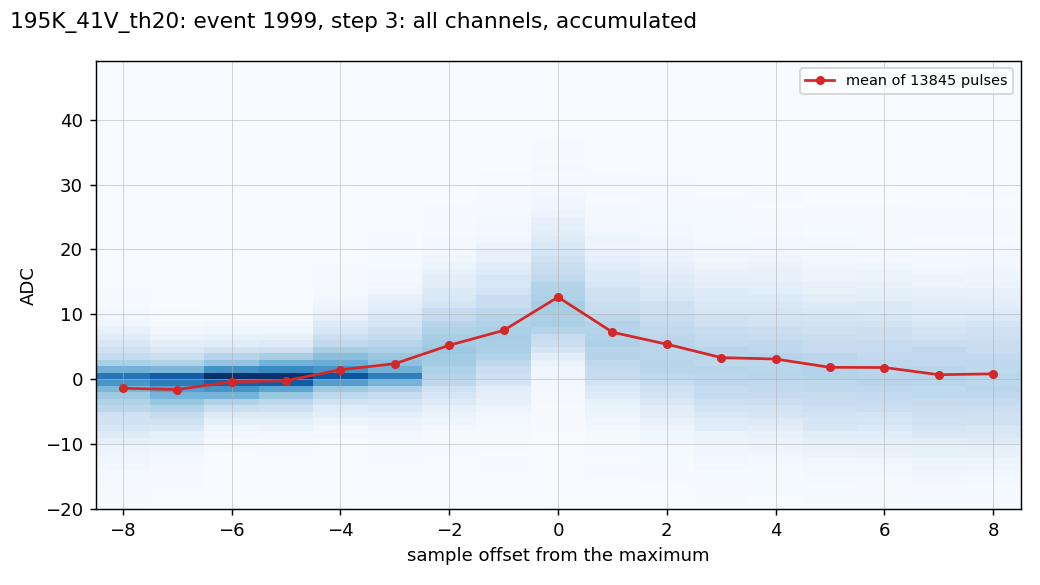
\includegraphics[width=0.8\textwidth]{../figs/tpl_195K_s3.png}\end{center}

The aligned pulses: the pre-peak samples sit at zero (the local
baseline), the pulse rises over two samples, peaks at 12.7 counts above
its local level (the threshold of 20 is on the raw value, which includes
that level), and decays over six samples; the spread after the peak is
wide, $\pm 10$ counts, from pulses riding on other pulses.

\paragraph{First template (step 4).}
\begin{lstlisting}
T1 = -0.108 -0.124 -0.030 -0.017 +0.117 +0.190 +0.414 +0.595 +1.000
     +0.573 +0.427 +0.264 +0.247 +0.146 +0.144 +0.056 +0.067
FWHM 3.03 samples (24 ns), undershoot +0.056, sum of squares 2.295
\end{lstlisting}
Identical, to the third decimal, to the template from the first 300
events: the shape is stable. The matched-filter gain is 1.51.

\begin{center}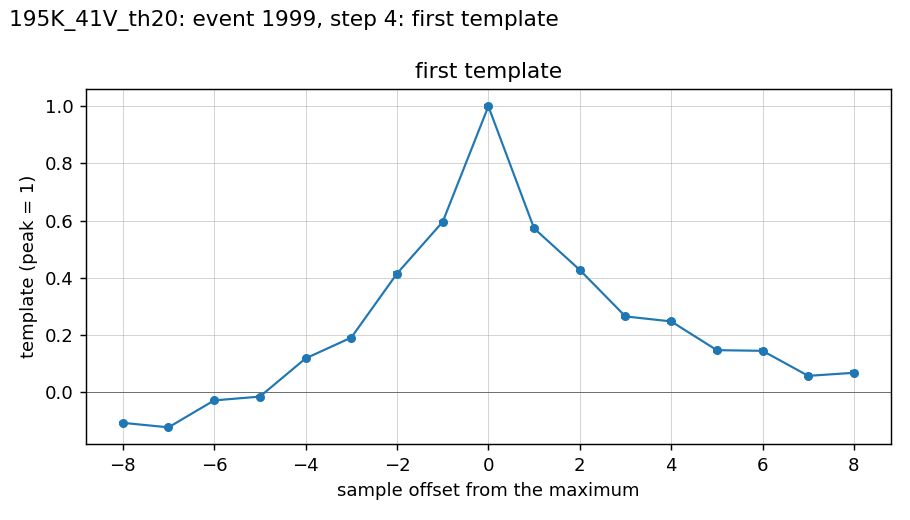
\includegraphics[width=0.6\textwidth]{../figs/tpl_195K_s4.png}\end{center}

\paragraph{Refined template (step 5).} 16\,335 pulses; $T^{(2)}$ has
the same rise but a tail twice as high ($+0.2$ at 8 samples against
$+0.07$), width 4.8 samples. The filtered selection, which weights the
tail, picks more of the pulses that have one (afterpulses, delayed
crosstalk, a second pulse close behind). The same happened in every
variant tried (alignment on the filtered maximum, a free constant in the
fit). $T^{(1)}$ is used.

\begin{center}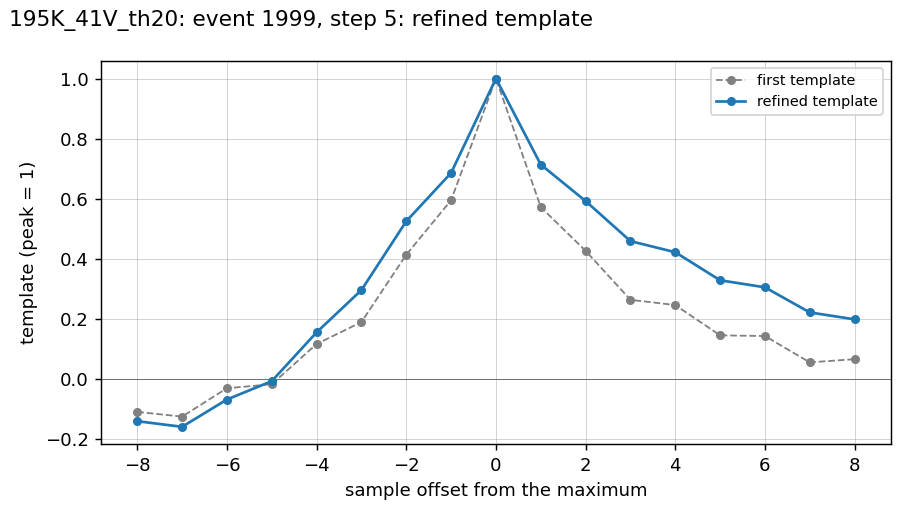
\includegraphics[width=0.6\textwidth]{../figs/tpl_195K_s5.png}\end{center}

\paragraph{Per-channel check (step 6).} Residual to the template, median
0.023 in peak units; channel 49 stands out (0.06), the others agree. One
template serves all channels that have pulses.

\begin{center}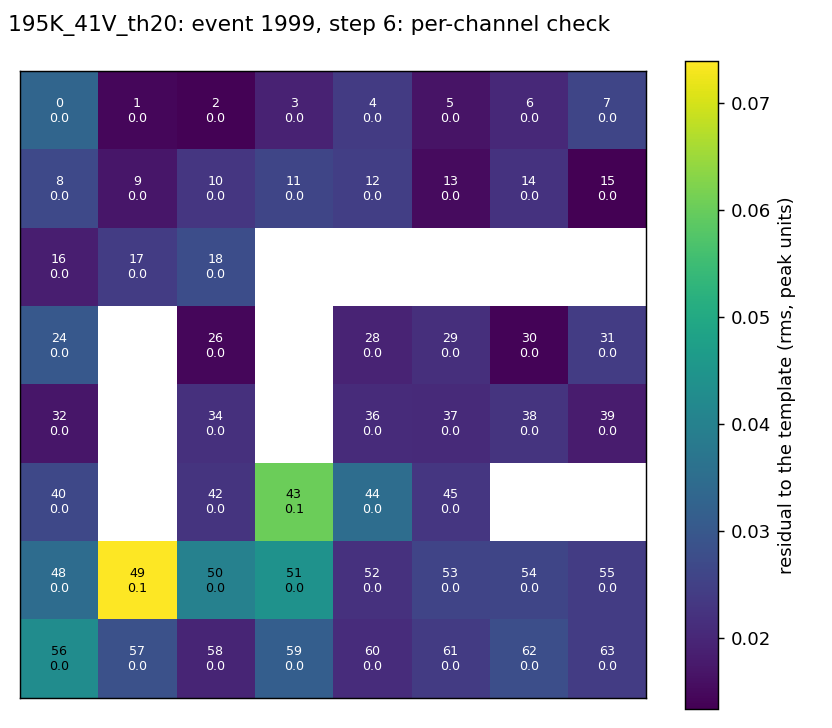
\includegraphics[width=0.6\textwidth]{../figs/tpl_195K_s6.png}\end{center}

\paragraph{Noise model and whitened filter (step 7, 500 events).}
\begin{lstlisting}
noise from 12 dead channels, 6000 segments of 1250 samples: rms 3.83 ADC;
autocorrelation rho(1..8) = +0.43 +0.16 +0.02 +0.02 +0.00 +0.03 +0.01 +0.03;
correlation length 2 samples; noise power below 10 / 20 / 30 MHz: 34% / 59% / 75%
predicted noise: single sample 3.83, matched filter 3.61 (white-noise expectation 2.52),
whitened filter (33 samples) 3.42; measured on the dead channels: matched 3.50,
whitened 3.28; gains over a single sample: matched 1.09, whitened 1.17
\end{lstlisting}
The noise is correlated over two samples (0.43 at one lag, 0.16 at two,
nothing beyond) and its spectrum is nearly flat, like the spectrum of
the template: the pulse occupies the same band as the noise. The
whitened filter gains 1.17 over a single sample, the matched filter
1.09, and the white-noise prediction of 1.5 is never reached. No linear
filter built on this pulse shape separates the single photoelectron
from the noise better than a factor 1.2, and the single photoelectron
stays a 5-sigma object at 41~V and a 4-sigma one at 39~V. The weak
oscillation of the autocorrelation at even lags is a small component
near 31~MHz, of no consequence.

\begin{center}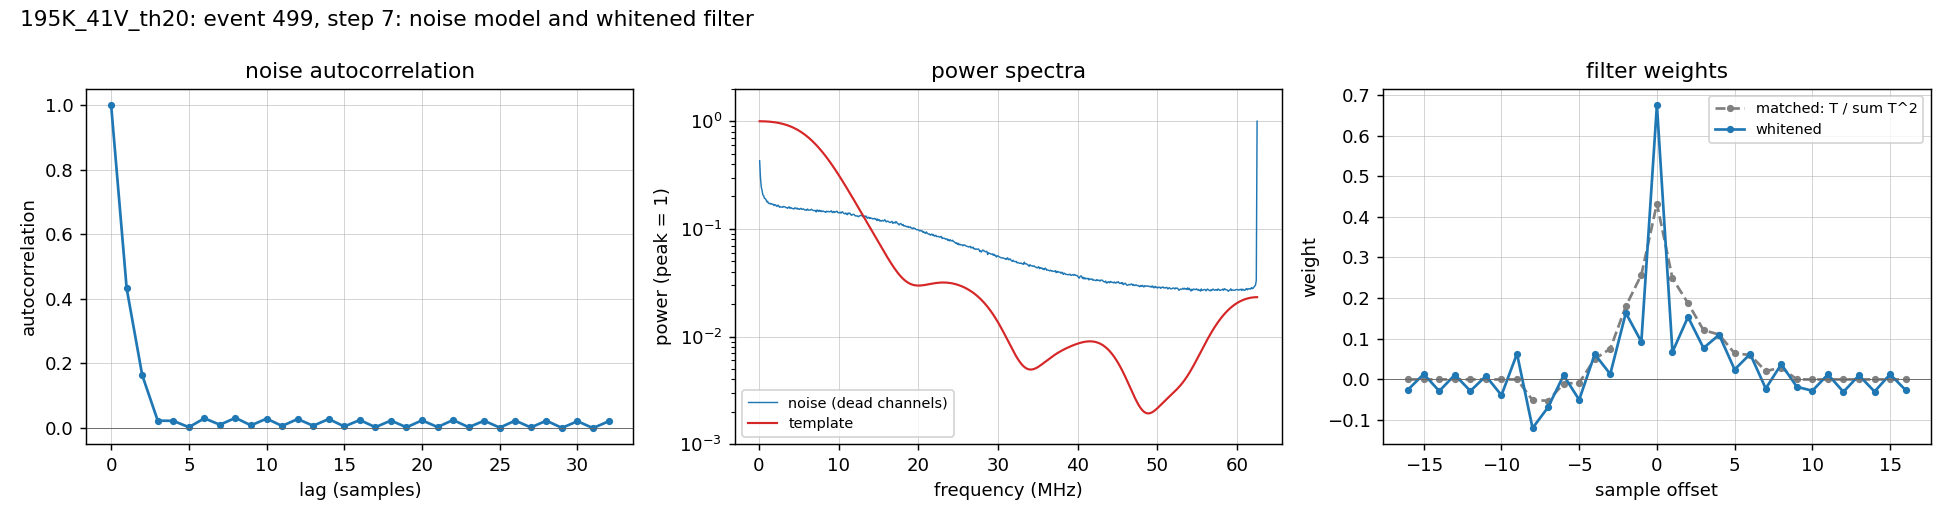
\includegraphics[width=\textwidth]{../figs/tpl_195K_s7.png}\end{center}

\section{Examples}

\begin{lstlisting}
# one event, channel 0, every step (the template from a handful of pulses)
python3 src/py/template.py 197K_39V_th20

# the template from 300 events, figures saved, template written
python3 src/py/template.py 197K_39V_th20 --events 0-299 --summary --save tpl197 \
        --write src/spe_template_197K_39V_th20.csv
\end{lstlisting}

\end{document}
